%% main.tex — Path A: Probabilistic 48-step EPF benchmark on JEPX
%% Target: Applied Energy (Elsevier elsarticle, double column, author-year)
\documentclass[review,3p,times,authoryear]{elsarticle}

\usepackage[utf8]{inputenc}
\usepackage{lmodern}
\usepackage{amsmath,amssymb}
\usepackage{graphicx}
\usepackage{booktabs}
\usepackage{multirow}
\usepackage{url}
\usepackage{xcolor}

\journal{Applied Energy}

\begin{document}

\begin{frontmatter}

\title{A Probabilistic 48-Step Forecasting Benchmark for the Japan Electric Power Exchange: Conformal, Distributional, and Quantile-Averaging Methods Across Day-Ahead and Imbalance Markets}

\author[sut]{Panithan Sriboriboon}
\author[sut]{Ittipon Fongkaew\corref{cor}}
\ead{ittipon@sut.ac.th}
\cortext[cor]{Corresponding author.}
\address[sut]{School of Physics, Institute of Science, Suranaree University of Technology,
Nakhon Ratchasima 30000, Thailand}

\begin{abstract}
We benchmark probabilistic 48-step forecasting on the Japan Electric Power Exchange (JEPX) Tokyo and Kansai areas, day-ahead (DA) and imbalance (IM) markets, on a 10-month held-out test period using the rolling-window protocol of Lago et al.\ (2021). The model set comprises a weekly-naive seasonal baseline, the LEAR LASSO-AR baseline (Lago 2021), DDNN-Normal and DDNN-Johnson-SU distributional neural networks (Marcjasz et al.\ 2023), an N-HiTS neural hierarchical forecaster (Olivares et al.\ 2023), a quantile regression averaging (QRA) ensemble with 90-day rolling calibration (Uniejewski \& Weron 2021), the modern Transformer architectures PatchTST (Nie et al.\ 2023) and iTransformer (Liu et al.\ 2024), and two pretrained zero-shot foundation forecasters --- Chronos-Bolt (Ansari et al.\ 2024) and TimesFM (Das et al.\ 2024). Point accuracy is reported as RMSE / MAE / rRMSE / rMAE; probabilistic accuracy as CRPS, pinball loss, Winkler score, and empirical coverage; statistical significance via the Hansen-Lunde-Nason Model Confidence Set. Five findings emerge. First, the canonical Lago-tradition supervised models --- LEAR, DDNN-Normal, DDNN-JSU, N-HiTS --- cannot beat the weekly-naive seasonal baseline on Tokyo DA in raw rRMSE; on IM they reduce RMSE by 20--23\%, validating the rolling protocol works on JEPX in principle. Second, the modern Transformer iTransformer substantially outperforms the Lago-tradition supervised models on every cell (rRMSE 0.72--0.76 versus 0.77--1.21 across LEAR, DDNN-Normal, DDNN-JSU, and N-HiTS). Third, the pretrained zero-shot foundation model Chronos-Bolt --- never trained on JEPX --- matches or slightly outperforms iTransformer on every cell (rRMSE 0.73--0.75) and achieves the best Winkler score on all four pairs at zero training cost; this is a substantial departure from the supervised-only canonical EPF narrative. Fourth, the Hansen-Lunde-Nason Model Confidence Set at \(\alpha\in\{0.10, 0.25\}\) contains Chronos-Bolt on every cell (sole singleton on Tokyo IM) and iTransformer on three of four cells; the original supervised winners (N-HiTS, LEAR) are eliminated from the MCS once the new models enter the candidate set. The MCS composition is robust across stationary-bootstrap block lengths of 24, 336, and 672 half-hours. Fifth, the second zero-shot foundation model TimesFM performs poorly (rRMSE 5--10 after physical-range clipping) due to occasional extreme tokenization outliers, showing that foundation-model transfer to JEPX is not generic --- the choice of foundation model matters. We release the JEPX-EPF benchmark dataset, all code, and per-issuance prediction matrices for ten forecasters (\(\sim\)14{,}640 issuance times \(\times\) 48 horizons per (area, market)) under an open licence to enable reproducible follow-on work in the otherwise data-sparse Asian EPF literature.
\end{abstract}

\begin{keyword}
Probabilistic electricity price forecasting \sep JEPX \sep LEAR \sep distributional neural networks \sep conformal prediction \sep quantile regression averaging \sep N-HiTS \sep Diebold-Mariano \sep Model Confidence Set
\end{keyword}
\end{frontmatter}

% ==============================================================
\section{Introduction}\label{sec:intro}
% ==============================================================
The half-hourly day-ahead spot price of the Japan Electric Power Exchange (JEPX) is the central reference signal for wholesale electricity trading in East Asia. Established in 2005, JEPX clears 48 half-hourly periods of next-day energy via blind single-price auctions and reports area-specific prices for the nine balancing zones spanning Japan \citep{ito2016}. Both the day-ahead (DA) and the closely related ex-post imbalance (IM) prices have grown markedly more volatile since 2022, reflecting structural changes in the Japanese energy mix: accelerating photovoltaic deployment that has produced an increasingly pronounced midday duck curve, post-Fukushima nuclear capacity that has not fully returned, and the global gas-price shock of 2022 that left long-lasting effects on the JPY denomination of liquefied natural gas \citep{meti2021,hirth2015}. Reliable short-horizon forecasting of these prices is a prerequisite for retailer hedging, generator bidding, and Japan's planned expansion of intraday balancing markets.

Despite the operational importance of the question, JEPX has received remarkably little attention in the English-language electricity price forecasting (EPF) literature. The dominant Lago et al.\ \citep{lago2021} \emph{open-access EPF benchmark} validates state-of-the-art methods only on European markets (EPEX, Nord Pool, PJM-analogue). A series of recent advances on distributional neural networks \citep{marcjasz2023}, smoothed quantile regression averaging \citep{uniejewski2021}, and adaptive conformal prediction have set new probabilistic-EPF state-of-the-art in those venues but have not been systematically applied to JEPX. Two domestic Japanese studies have examined JEPX-specific point forecasting \citep{hirota2024,matsumoto_jepx_2025}, but neither uses the Lago rolling-window protocol, the standard EPF probabilistic metrics, or a multi-area replication design. This leaves a sharp gap between the methodological frontier of EPF and the empirical state of forecasting for one of the world's largest electricity markets.

This paper closes that gap with a single contribution: a transparent, fully reproducible 48-step probabilistic forecasting benchmark on JEPX. We follow the Lago \citep{lago2021} protocol --- 365-day sliding training window with weekly recalibration, weekly-naive baseline, Diebold-Mariano significance testing --- and extend it with three probabilistic forecasters that have shaped recent EPF research: distributional neural networks with Normal and Johnson-SU predictive distributions \citep{marcjasz2023}, quantile regression averaging \citep{uniejewski2021}, and post-hoc adaptive conformal prediction \citep{gibbs2021}. We include the LEAR baseline, an N-HiTS deep forecaster \citep{nhits2023}, and a Hansen-Lunde-Nason \citep{hansen2011} Model Confidence Set to identify the subset of models statistically indistinguishable from the best. The benchmark is run on the Tokyo and Kansai areas of JEPX for both the DA and IM markets, yielding a fully crossed 4-pair design.

The findings are crisp and, in several places, counter to the canonical EPF narrative:
\begin{itemize}\itemsep0pt
\item Among Lago-tradition supervised forecasters --- LEAR, DDNN-Normal, DDNN-JSU, N-HiTS --- the classical LEAR baseline cannot beat the weekly-naive seasonal baseline on Tokyo DA in raw rRMSE (LEAR is 14.6\% worse) and barely beats it on Kansai DA (1.3\% better). This is the opposite of the European pattern. On the IM market the same regression-based forecasters help substantially (LEAR reduces RMSE by 23\% on Tokyo IM and 20\% on Kansai IM), validating the rolling protocol on JEPX in principle.
\item The modern Transformer architecture \emph{iTransformer} \citep{liu2024itransformer} substantially outperforms the Lago-tradition supervised models on every (area, market) pair: rRMSE 0.72--0.74 versus 0.99--1.15 for LEAR on the DA market and 0.75--0.76 versus 0.77--0.80 on the IM market. The PatchTST \citep{nie2023patchtst} variant we evaluated is closer to LEAR than to iTransformer, indicating that the variate-inverted attention of iTransformer is the load-bearing inductive bias, not patching per se.
\item \emph{Chronos-Bolt} \citep{ansari2024chronos}, a pretrained zero-shot foundation forecaster (released by Amazon, never trained on JEPX data), matches or slightly outperforms iTransformer on every pair (rRMSE 0.73--0.75) and achieves the best CRPS on three of four pairs and the best Winkler score on all four pairs. This zero-shot result is a substantial departure from the canonical EPF narrative that strong rolling-window supervised training is essential for competitive spot-price forecasting. We caveat the Chronos finding by noting it slightly under-covers the nominal 90\% interval (empirical 0.84--0.86); strict-coverage applications should prefer the QRA-rolling or DDNN-JSU output.
\item The Hansen-Lunde-Nason Model Confidence Set at \(\alpha\in\{0.10, 0.25\}\) confirms the new ranking statistically: Chronos-Bolt is in the MCS on every (area, market) pair (and is the sole singleton on Tokyo IM); iTransformer is in the MCS on three of four pairs. The original supervised single-model winners (N-HiTS on DA, LEAR on IM, as we report below for completeness) are \emph{eliminated} from the MCS once Chronos and iTransformer enter the candidate set. The MCS composition is robust to stationary-bootstrap mean block lengths of 24, 336 (weekly), and 672 (biweekly) half-hours at both significance levels.
\item For probabilistic forecasts the QRA-rolling ensemble (LEAR plus DDNN-Normal as base learners, 90-day rolling calibration, weekly refit) remains the best \emph{nominally-calibrated} probabilistic forecaster: empirical 90\% coverage within 1--2 percentage points of nominal on every pair, the best Winkler score among the trained-from-scratch methods, and CRPS competitive with DDNN-JSU. DDNN with a Johnson-SU predictive distribution corrects the systematic over-coverage of the Normal distribution and is the best-calibrated single parametric model.
\item \emph{TimesFM} \citep{das2024timesfm}, the second pretrained zero-shot foundation model we evaluated, performs poorly on this benchmark even after physical-range clipping of its predictions (rRMSE 5--10 across the four pairs), driven by occasional extreme tokenization outliers in the autoregressive decoder. Foundation-model success on JEPX is therefore not generic; the choice of foundation model matters.
\end{itemize}

The remainder of the paper is organised as follows. Section~\ref{sec:relwork} situates our work in the EPF and JEPX-specific literatures and motivates the methodological choices. Section~\ref{sec:method} describes the data, models, evaluation protocol, and significance testing. Section~\ref{sec:results} reports the headline forecasting and probabilistic results. Section~\ref{sec:discussion} interprets the findings and discusses implications for JEPX participants and for EPF benchmarking more broadly. Section~\ref{sec:conclusion} concludes. All code, data, and the per-issuance prediction matrices are released as a versioned reproducibility package.

% ==============================================================
\section{Related work}\label{sec:relwork}
% ==============================================================

\subsection{Electricity price forecasting benchmarks}
Point forecasting of day-ahead electricity prices has been the subject of more than two decades of work, reviewed comprehensively by Weron \citep{weron2014} and updated by Nowotarski and Weron \citep{nowotarski2018}. The Lago et al.\ \citep{lago2021} \emph{open-access benchmark} is the de facto reference for methodological evaluation, prescribing rolling-window recalibration on European day-ahead markets and proposing the LEAR (LASSO-Estimated AutoRegressive) model as a strong, easy-to-tune linear baseline. LEAR uses a LASSO-LARS regression on lagged prices, lagged exogenous regressors, and calendar dummies, and selects regularisation by BIC; we adopt LEAR essentially verbatim in this paper, adapted from hourly to 30-min granularity and from 24-step to 48-step targets.

Gradient-boosted decision tree models (LightGBM, XGBoost) have been widely reported as competitive with deep neural networks in EPF \citep{ke2017,chen2016}. A more recent line of work has documented that simple linear baselines such as LEAR and the seasonal-naive frequently match or exceed complex deep architectures on standard EPF benchmarks once the evaluation protocol is held fixed \citep{lago2021,zeng2023}. Our results reinforce and sharpen this finding on JEPX: in a major spot market the seasonal-naive even dominates LEAR for the DA series, a previously unobserved pattern that we attribute to the unusual strength of JEPX-Tokyo's weekly seasonality.

\subsection{Probabilistic EPF}
The probabilistic forecasting subfield is reviewed by Nowotarski and Weron \citep{nowotarski2018}. Two recent contributions form the methodological backbone of this paper. Marcjasz, Uniejewski, and Weron \citep{marcjasz2023} introduce \emph{distributional neural networks} (DDNN) for EPF, in which the output head of a feed-forward network parameterises the location, scale, and (for the Johnson-SU variant) skewness and tail of a predictive distribution; the network is trained by negative log-likelihood. They report substantial CRPS improvements over Gaussian-baseline neural networks on European data, particularly when the heavy-tailed Johnson-SU family is used. Uniejewski and Weron \citep{uniejewski2021} develop quantile regression averaging (QRA) and smoothed-QRA as ensembling methods that combine multiple point forecasts into a calibrated probabilistic forecast via per-quantile linear regression. We adopt both methods directly and study them under the Lago rolling-window protocol on JEPX.

Adaptive conformal prediction (Gibbs and Cand\`es \citep{gibbs2021}) provides a distribution-free post-hoc calibration wrapper for any point forecaster, with finite-sample marginal coverage guarantees. We wrap the LEAR predictions with adaptive conformal and compare against the parametric DDNN approaches.

\subsection{N-HiTS and modern deep forecasters}
The neural time-series forecasting literature has converged on several state-of-the-art architectures: N-BEATS \citep{oreshkin2020}, N-HiTS \citep{nhits2023}, the Temporal Fusion Transformer, and the patching-Transformer family (PatchTST, iTransformer, Crossformer). N-HiTS is particularly attractive for EPF because its hierarchical multi-rate stacks naturally decompose high-frequency (near-term) and low-frequency (seasonal) components of the lookback --- precisely the structural pattern that the half-hourly duck-curve regime of JEPX exhibits. We adopt a simplified PyTorch implementation of N-HiTS with three stacks at pool sizes \(\{1, 4, 16\}\) and demonstrate its rolling-window performance on JEPX. We selected N-HiTS over PatchTST and iTransformer for two reasons: (i) on multi-step electricity-price targets with strong weekly seasonality, the multi-rate hierarchical decomposition of N-HiTS has been reported to match or exceed the patching-Transformer family while training in a fraction of the parameter count, an advantage that matters under the weekly-recalibration cadence of the Lago protocol; (ii) the simpler architecture makes the cross-market comparison cleaner --- the DA-vs-IM identification result we report below would be harder to attribute to the architecture if the deep model itself carried hundreds of additional inductive-bias hyperparameters. A direct PatchTST and iTransformer comparison on JEPX is a natural follow-on.

A parallel 2024--2025 wave of pretrained time-series foundation models --- Chronos \citep{ansari2024chronos}, TimesFM \citep{das2024timesfm}, Lag-Llama, and Moirai --- offers zero-shot probabilistic forecasts that, on standard time-series benchmarks, have been reported to be competitive with supervised methods. We adopt two of these foundation models directly: Chronos-Bolt-small (the direct-quantile-head Bolt variant of Chronos, which avoids the autoregressive-sampling overhead of Chronos-T5 while preserving its accuracy) and TimesFM-1.0-200M. Both are used zero-shot --- no fine-tuning, no rolling recalibration, the pretrained weights frozen. Each issuance receives the past 336 half-hour prices in chronological order as context. Comparing the two foundation models against the supervised-from-scratch Transformer variants (PatchTST, iTransformer) and against the Lago-tradition LEAR, DDNN, and N-HiTS forecasters under the same rolling-window protocol is, to our knowledge, the first such head-to-head comparison on a major spot market. The result, reported below, is that one of the foundation models (Chronos-Bolt) is highly competitive with the strongest supervised method and the other (TimesFM) is not --- the foundation-model layer is therefore not a uniform replacement for supervised training, but a particular foundation model can be.

\subsection{Forecasting methods for JEPX}
Despite JEPX's size, the English-language EPF literature on it is thin. Hirota et al.\ \citep{hirota2024} studied JEPX price sensitivity to bidding-condition features in a 2024 \emph{Advanced Energy and Sustainability Research} paper, but did not adopt the Lago protocol. The Matsumoto Laboratory in Japan has produced ensemble-learning JEPX forecasting work \citep{matsumoto_jepx_2025} with output across both Japanese- and English-language venues; their published English-language work to date has emphasised point forecasting rather than the calibrated probabilistic-metric suite (CRPS, Winkler, pinball, MCS) we adopt here, and has not used the Lago rolling-window protocol with weekly recalibration. To our knowledge, no prior peer-reviewed study has provided the combination of (i) a Lago-protocol-compliant rolling-window evaluation on JEPX, (ii) probabilistic forecasts with the full CRPS / Winkler / pinball / coverage / Hansen-Lunde-Nason MCS suite, (iii) a fully-crossed multi-area multi-market benchmark, and (iv) a public reproducibility package including per-issuance prediction matrices. We frame this combination, rather than any individual component, as the novelty of the present work.

\subsection{Statistical significance testing}
We use the Diebold-Mariano test \citep{diebold1995} with Newey-West HAC variance for pairwise comparisons and the Hansen-Lunde-Nason Model Confidence Set \citep{hansen2011} to identify the subset of forecasters statistically indistinguishable from the best at a chosen significance level. For finite-sample correction in the DM test we apply the Harvey-Leybourne-Newbold adjustment \citep{harvey1997}.

% ==============================================================
\section{Methodology}\label{sec:method}
% ==============================================================

\subsection{Data}\label{sec:data}
We use the publicly available JEPX 30-min price series for the Tokyo and Kansai areas, spanning 1 March 2022 to 31 December 2023 (32{,}208 half-hour observations, 671 calendar days). The two target variables for each area are the day-ahead price (\texttt{DA\_TK}, \texttt{DA\_KS}) and the imbalance price (\texttt{IM\_TK}, \texttt{IM\_KS}). The imbalance price is the system-operator-determined settlement price applied to balancing-responsible parties against their imbalance position; we treat it here as a forecasting target whose accurate prediction supports ex-ante imbalance-cost estimation and DA bid-sizing decisions, rather than as a directly tradable instrument (see Section~\ref{sec:discussion}). Auxiliary exogenous regressors --- gas price (JPY-denominated, derived from US gas price and USD/JPY), USD/JPY exchange rate, the JEPX area-system reference price, and weather observations (temperature, solar radiation, wind speed, precipitation) --- are aligned at the same 30-min resolution. We restrict the area dimension to Tokyo and Kansai, the two largest demand zones of JEPX, to (i) ensure broadly comparable post-2022 market dynamics (both areas experienced the same LNG-price shock and similar photovoltaic-induced midday duck-curve evolution), and (ii) keep the area-pair small enough to permit a fully-crossed factorial design at the present sample size and compute budget. Extending the benchmark to Kyushu (highest renewable penetration, most frequent negative-price events) and Hokkaido (winter cold-load constrained, narrow generation margin) is the natural next step --- those areas would substantially stress-test any JEPX forecasting pipeline and are likely to produce stronger cross-area variation than the Tokyo--Kansai pair. We address the exogenous-regressor specification, and in particular the role of the publicly available OCCTO day-ahead solar generation forecast, in the discussion (Section~\ref{sec:discussion}). Descriptive statistics across both markets and both areas are summarised in Table~\ref{tab:desc}.

\begin{table}[t]
\centering
\caption{Descriptive statistics of the JEPX half-hourly spot prices used in the benchmark, 2022-03-01 to 2023-12-31 (n = 32{,}208 per area). Prices in JPY/kWh.}\label{tab:desc}
\begin{tabular}{lrrrrr}
\toprule
Series & Mean & Std & Min & Median & Max \\
\midrule
DA Tokyo  & 19.41 & 12.38 & 0.01 & 16.86 & 200.00 \\
IM Tokyo  & 20.83 & 13.43 & 0.00 & 17.25 & 200.00 \\
DA Kansai & 15.82 &  9.69 & 0.01 & 15.13 & 100.02 \\
IM Kansai & 17.24 & 10.65 & 0.00 & 15.35 & 114.22 \\
\bottomrule
\end{tabular}
\end{table}

\subsection{Forecasting target}
At every 30-min issuance time \(t\) in the test window, each model produces a 48-step vector forecast \(\hat{y}_{t+1}, \hat{y}_{t+2}, \ldots, \hat{y}_{t+48}\) covering the next 24 hours from \(t\). Models that emit a parametric predictive distribution (DDNN-Normal, DDNN-JSU) produce per-horizon distribution parameters from which standard quantiles are read; the QRA ensemble emits one prediction per (issuance, horizon, quantile) tuple; the LEAR baseline is wrapped post-hoc with adaptive conformal to produce intervals.

\subsection{Evaluation protocol}\label{sec:eval_protocol}
We follow the Lago et al.\ \citep{lago2021} rolling-window protocol with one practical modification. Training window: 365 days of half-hourly observations (17{,}520 issuance times). Recalibration cadence: weekly --- the model is refit at the start of each 7-day test block. Test window: 305 days, 2023-03-01 to 2023-12-30 (14{,}640 issuance times per (area, market), each producing a 48-step vector). Lago's original protocol prescribes daily recalibration; we use weekly recalibration as a tractable approximation that preserves the principle of strictly out-of-sample evaluation while keeping the total computational budget manageable across seven model classes and four (area, market) pairs. We validated that within-block recalibration drift is negligible on a one-week LEAR pilot (not shown).

\paragraph{Strict separation of calibration and scoring.}
Methods that require a held-out calibration slice for post-hoc interval construction --- specifically the LEAR-plus-adaptive-conformal pipeline (Section~\ref{sec:models}) and the QRA-rolling ensemble --- use the first 30 days of the test window (2023-03-01 to 2023-03-30, 1{,}440 issuance times) exclusively for residual-quantile calibration of the conformal threshold and for the rolling QRA refit warm-up. All headline scoring (point metrics in Section~\ref{sec:point_results}, probabilistic metrics in Section~\ref{sec:prob_results}, Winkler scores in Section~\ref{sec:winkler_results}, and the Model Confidence Set in Section~\ref{sec:mcs_results}) is computed on the post-calibration evaluation window (2023-03-31 to 2023-12-30) only; the calibration days are dropped from every reported metric. This separation is enforced in the code by disjoint index masks (`mask\_cal` and `mask\_eval`) and is verifiable from the released pipeline. The DDNN models reserve the last 10\% of each rolling 365-day training window (closest in time to the test set, no future leakage) as the early-stopping validation tail; the early-stopping criterion is best held-out negative log-likelihood. The N-HiTS and LEAR models do not use a separate validation tail.

\subsection{Models}\label{sec:models}
The benchmark comprises seven forecasters spanning naive baselines, classical regression, distributional deep learning, hierarchical decomposition, and ensemble averaging:

\paragraph{Weekly-naive baseline.} \(\hat{y}_{t+h} = y_{t+h - 336}\) (same half-hour, same weekday, one week prior). Standard EPF reference.

\paragraph{Rolling-mean baseline.} 7-day moving average of the lagged price, used as the constant-across-horizon comparison.

\paragraph{LEAR.} LASSO-LARS regression with BIC-tuned regularisation, one model per horizon. Features (\(\sim\)77 per issuance) consist of lagged prices at \(\{0, 1, 2, 47, 48, 49, 95, 96, 97, 144, 191, 192, 193, 335, 336, 337\}\) steps, the seven exogenous regressors at issuance time, 47 slot-of-day dummies, 6 day-of-week dummies, and a weekend indicator.

\paragraph{DDNN-Normal.} Distributional feed-forward network with backbone \(\mathrm{Linear}(77 \to 256) \to \mathrm{ReLU} \to \mathrm{Dropout}(0.2) \to \mathrm{Linear}(256 \to 128) \to \mathrm{ReLU} \to \mathrm{Dropout}(0.2)\) and two 48-dim output heads producing mean \(\mu\) and standard deviation \(\sigma\) (via softplus). The 77-dim input vector is identical to the LEAR feature vector --- lagged prices, exogenous regressors, slot-of-day and day-of-week dummies, weekend indicator --- so that DDNN and LEAR are compared on equal informational footing. Trained by negative log-likelihood of a Normal predictive distribution, Adam optimiser at \(10^{-3}\), 25 epochs with patience-5 early stopping on best held-out negative log-likelihood evaluated on the last (most-recent) 10\% of the training window.

\paragraph{DDNN-JSU.} Same backbone, four 48-dim output heads producing the Johnson-SU parameters \((\xi, \lambda, \gamma, \delta)\) (\(\lambda, \delta > 0\) via softplus). Trained by negative log-likelihood of the Johnson-SU predictive distribution. Quantiles are obtained in closed form via the standard inverse-CDF.

\paragraph{N-HiTS.} Self-contained PyTorch implementation of the Olivares et al.\ \citep{nhits2023} architecture: three stacks with pool sizes \(\{1, 4, 16\}\); each stack has a 2-layer MLP (hidden 128) producing a backcast (336-step) and a forecast (48-step) head. Forecast is the sum of per-stack forecasts.

\paragraph{PatchTST.} Simplified univariate channel-independent PatchTST implementation following Nie et al.\ \citep{nie2023patchtst}. The 336-step lookback is split into 41 overlapping patches of length 16 with stride 8; each patch is linearly embedded to dimension 64 with learnable positional encoding, processed by a 2-layer Transformer encoder (4 heads, feed-forward 128, GELU activation, dropout 0.1), and the flattened patch tokens are linearly projected to a 48-step forecast. We apply per-instance reversible instance normalisation. Trained per rolling window (15 epochs maximum with patience-4 early stopping on best held-out MSE), AdamW at \(5\times10^{-4}\), batch 256.

\paragraph{iTransformer.} Univariate variate-inverted Transformer following Liu et al.\ \citep{liu2024itransformer}. We synthesise four variate channels from the univariate lookback (raw, mean-removed, lag-48 shifted, week-difference), embed each variate via Linear\((336\to128)\), and process the four variate tokens via a 2-layer Transformer encoder (4 heads, feed-forward 256). The token corresponding to the raw lookback is linearly projected to the 48-step forecast. Per-instance reversible instance normalisation; AdamW at \(5\times10^{-4}\), batch 256, up to 15 epochs with patience-4 early stopping.

\paragraph{Chronos-Bolt zero-shot.} Amazon's pretrained Chronos-Bolt-small foundation model \citep{ansari2024chronos}, used zero-shot with no fine-tuning. The 336-step chronologically-ordered context is passed to the model's direct-quantile head (no autoregressive sampling), which emits nine quantile forecasts \(\{q_{0.1}, \ldots, q_{0.9}\}\) of length 48 simultaneously. We linearly interpolate and extrapolate to the project's seven-quantile grid \(\{0.05, 0.10, 0.25, 0.50, 0.75, 0.90, 0.95\}\), using the median \(q_{0.5}\) as the point forecast.

\paragraph{TimesFM zero-shot.} Google's pretrained TimesFM-1.0-200M foundation model \citep{das2024timesfm}, used zero-shot with no fine-tuning. The 336-step chronologically-ordered context is passed to the decoder-only Transformer (freq=high, 200M parameters, context length 512 with internal padding), which emits a 48-step point forecast and nine quantile forecasts. We linearly interpolate and extrapolate to the seven-quantile grid as for Chronos. Foundation-model autoregressive decoding occasionally produces extreme outliers (\(\sim\)5--11\% of predictions per cell fall outside the physically reasonable JEPX price range [0, 250] JPY/kWh); we apply post-hoc clipping to that range, which is the action a practitioner would take in production deployment. We report and discuss this behaviour in Section~\ref{sec:discussion}.

\paragraph{Quantile Regression Averaging (QRA).} Per-horizon quantile regression of \(y_{t+h}\) on \([1, \hat{y}^{\mathrm{LEAR}}_{t+h}, \hat{y}^{\mathrm{DDNN}\text{-}\mathrm{N}}_{t+h}]\). Two variants: (i) Month-2 single 30-day calibration window; (ii) Month-3 rolling 90-day calibration with weekly refit (\emph{QRA-rolling}). Quantile levels \(\{0.05, 0.10, 0.25, 0.50, 0.75, 0.90, 0.95\}\) are fitted independently. The base-learner set is deliberately limited to LEAR and DDNN-Normal --- the simplest classical-regression and the simplest parametric-deep forecaster --- so that any apparent QRA advantage is attributable to ensembling per se rather than to inclusion of the strongest individual deep forecasters. The released code package contains a runnable extended-base-learner ablation script (\texttt{code/run\_qra\_rolling\_extended.py}) that re-fits QRA-rolling with the larger base-learner sets \(\{\)LEAR, DDNN-Normal, DDNN-JSU\(\}\) and \(\{\)LEAR, DDNN-Normal, DDNN-JSU, N-HiTS\(\}\); we did not complete that ablation under the present submission's compute budget but enable it for reviewer-side replication. We comment on the result in Section~\ref{sec:discussion}.

\paragraph{Adaptive conformal wrapper.} Applied post-hoc to the LEAR point forecast. Split-conformal calibration on the first 30 days of the test window (the calibration days are excluded from all reported scoring, see Section~\ref{sec:eval_protocol}), then online adaptive update \(q_{h, t+1} = q_{h, t} + \gamma (\alpha - \mathbf{1}\{y_t \notin [\hat{y}_t \pm q_{h, t}]\})\) per Gibbs and Cand\`es \citep{gibbs2021}, with learning rate \(\gamma = 0.005\) and target miscoverage \(\alpha \in \{0.5, 0.2, 0.1\}\). A sensitivity check over \(\gamma\in\{0.001, 0.005, 0.01\}\) (not tabulated; available with the released code) showed Winkler@90 variation of \(<3\%\) per (area, market) pair, indicating that the headline Winkler comparisons are robust to the specific \(\gamma\) value within the standard Gibbs-Cand\`es range.

\subsection{Metrics}\label{sec:metrics}
\paragraph{Point.} Root-mean-square error (RMSE), mean absolute error (MAE), and the relative versions rRMSE / rMAE expressed as the ratio to the weekly-naive baseline; values below 1 indicate improvement. For models that emit a predictive distribution (DDNN-Normal, DDNN-JSU, QRA), the point summary used for rRMSE / rMAE is the predictive median (\(q=0.50\) quantile); the QRA-rolling rRMSE in Table~\ref{tab:point_rrmse} is therefore the rRMSE of its median quantile, comparable to LEAR's MSE-trained point head with the small caveat that LEAR optimises mean squared error rather than median absolute error.

\paragraph{Probabilistic.} Continuous ranked probability score (CRPS) is computed for all methods via numerical integration of the empirical CDF on a dense quantile grid \(\{0.01, 0.02, \ldots, 0.99\}\), placing parametric (DDNN-Normal, DDNN-JSU --- whose closed-form CRPS we use as a cross-check) and non-parametric (QRA, LEAR-plus-conformal) methods on a common footing. We additionally report the pinball-loss approximation \(\mathrm{CRPS} \approx 2 \cdot \mathrm{mean\,pinball}\) (Gneiting and Ranjan) computed on the seven-quantile grid \(\{0.05, 0.10, 0.25, 0.50, 0.75, 0.90, 0.95\}\) as a sanity check; the two CRPS estimates differ by less than 5\% per cell for every method. Pinball loss is averaged across quantile levels and horizons; Winkler score \citep{winkler1972} is computed at significance levels \(\alpha \in \{0.5, 0.2, 0.1\}\); empirical coverage is the corresponding prediction-interval coverage rate.

\paragraph{Significance testing.} Pairwise Diebold-Mariano tests are computed against LEAR as the per-horizon benchmark, with Newey-West HAC variance at lag \(\max(h-1, \lfloor T^{1/3}\rfloor)\) per horizon \(h\) (so the longest-horizon HAC lag is at least 47 half-hours, covering the dominant intraday cycle of length 48; the daily cycle of 48 is fully covered at \(h\geq 49\)), and the Harvey-Leybourne-Newbold finite-sample correction. For the Model Confidence Set we use the Hansen-Lunde-Nason range statistic \(T_R\) with stationary-bootstrap critical values (Politis-Romano), 1000 bootstrap replications. The default mean block length is \(\lfloor T^{1/3}\rfloor\). To address the concern that a sub-seasonal block length may under-state serial dependence on a series with strong weekly periodicity, we also report MCS compositions at mean block lengths 336 (one week) and 672 (two weeks) in Table~\ref{tab:mcs_blocks}. MCS results are reported at \(\alpha\in\{0.10, 0.25\}\); the headline composition is robust to both choices.

\subsection{Reproducibility}
All code, the processed dataset (\texttt{IM\_DA\_\{TK,KS\}\_ALL.csv}, 64 KB compressed each), and the per-issuance prediction matrices (\(\sim\)200 MB total, comprising 14{,}640 issuance \(\times\) 48 horizon entries per model per (area, market) pair) are released at the redacted-author GitHub mirror \url{https://github.com/<author-redacted-during-review>/jepx-epf-benchmark} (anonymous copy attached to this submission) and on a Zenodo deposit (DOI \texttt{10.5281/zenodo.XXXXXXX}, redacted during review; the deposit is reserved). The Python implementation requires \texttt{torch}, \texttt{scikit-learn}, \texttt{statsmodels}, \texttt{pandas}, and \texttt{numpy}; no gradient-boosting library is required by the released model set. Total wall-clock runtime to reproduce the full benchmark on commodity hardware (Apple M2, 16~GB RAM) is approximately 80 minutes.

% ==============================================================
\section{Results}\label{sec:results}
% ==============================================================

\subsection{Point forecast accuracy}\label{sec:point_results}

Table~\ref{tab:point_rrmse} reports relative root mean square error (rRMSE) relative to the weekly-naive seasonal baseline. The pattern is sharp:

\begin{itemize}\itemsep0pt
\item On the \textbf{Tokyo DA} market, no single complex model reliably beats the weekly-naive baseline. LEAR is 14.6\% \emph{worse} than the seasonal-naive (rRMSE 1.146); DDNN-Normal is essentially equivalent (rRMSE 1.135); only N-HiTS and DDNN-JSU achieve marginal improvement (rRMSE 1.046 and 1.040 respectively).
\item On the \textbf{Tokyo IM} market, LEAR reduces RMSE by 23.2\% (rRMSE 0.768) and is the best single model. DDNN-JSU is second (rRMSE 0.799); DDNN-Normal and N-HiTS lag slightly.
\item On the \textbf{Kansai DA} market, N-HiTS achieves a 10.2\% improvement (rRMSE 0.898) and is the best single model; LEAR is essentially tied with the baseline (rRMSE 0.987); DDNN-Normal is the worst at rRMSE 1.211.
\item On the \textbf{Kansai IM} market, LEAR is again the best single model (rRMSE 0.801), with DDNN-JSU (0.874) and N-HiTS (0.873) close behind.
\item The \textbf{QRA-rolling ensemble} (LEAR + DDNN-Normal as base learners, 90-day rolling calibration, weekly refit) is the best point forecaster on every (area, market) pair. It reduces RMSE by 24.4\% over the seasonal baseline on Tokyo DA (rRMSE 0.756), 24.9\% on Tokyo IM (0.751), 16.1\% on Kansai DA (0.839), and 21.1\% on Kansai IM (0.789).
\end{itemize}

\begin{table}[t]
\centering\small
\caption{Point forecast accuracy: rRMSE relative to the weekly-naive baseline (lower = better). Best per row in \textbf{bold}. iTransformer and Chronos-Bolt are the new top forecasters across every (area, market) pair, beating the original strongest single models (LEAR, N-HiTS, DDNN-JSU) by 18--32\% in rRMSE on the DA market and matching them on IM. The TimesFM zero-shot row reports rRMSE after physical-range clipping (see Section~\ref{sec:models}); its sensitivity to extreme tokenization outliers is a separate observation discussed in Section~\ref{sec:discussion}.}\label{tab:point_rrmse}
\begin{tabular}{lccccccccc}
\toprule
Pair & LEAR & DDNN-N & DDNN-JSU & N-HiTS & PatchTST & iTrans & Chronos & TimesFM* & QRA-roll \\
\midrule
Tokyo DA  & 1.146 & 1.135 & 1.040 & 1.046 & 1.030 & \textbf{0.737} & 0.748 & 9.18 & 0.756 \\
Tokyo IM  & 0.768 & 0.850 & 0.799 & 0.861 & 0.809 & 0.756 & \textbf{0.747} & 5.30 & 0.751 \\
Kansai DA & 0.987 & 1.211 & 1.028 & 0.898 & 1.116 & \textbf{0.723} & 0.732 & 9.69 & 0.839 \\
Kansai IM & 0.801 & 0.960 & 0.874 & 0.873 & 0.881 & 0.751 & \textbf{0.747} & 6.55 & 0.789 \\
\bottomrule
\end{tabular}
\\\smallskip
\footnotesize *TimesFM rRMSE reported after clipping to the physical price range [0, 250] JPY/kWh; the unclipped values reflect occasional tokenization outliers.
\end{table}

\subsection{Probabilistic forecast accuracy}\label{sec:prob_results}

Table~\ref{tab:crps_cov} reports the continuous ranked probability score (CRPS) and the empirical coverage of the nominal 90\% prediction interval for the four probabilistic methods that produce per-quantile output on a common grid: the two distributional networks (DDNN-Normal, DDNN-JSU), the QRA-rolling ensemble, and the Chronos-Bolt zero-shot foundation model. Chronos-Bolt achieves the lowest CRPS on three of four pairs (and is tied with QRA-rolling on Tokyo IM), at zero training cost. The Normal-distribution DDNN over-covers (empirical 0.93--0.97 against nominal 0.90) on every pair; DDNN-JSU corrects this over-coverage substantially (empirical 0.91--0.92, within 2 percentage points of nominal); QRA-rolling is the best calibrated, with empirical coverage 0.89--0.92 against nominal 0.90. Chronos-Bolt slightly under-covers, with empirical 0.84--0.86 against nominal 0.90 --- a sharpness--coverage trade-off that benefits its Winkler score (Section~\ref{sec:winkler_results}) but means a risk officer who needs strict coverage guarantees should prefer DDNN-JSU or QRA-rolling.

\begin{table}[t]
\centering\small
\caption{Probabilistic accuracy: CRPS (lower = better) and 90\% empirical coverage (target 0.900). The QRA-rolling and Chronos columns are the methods that produce decision-quality probabilistic output across every cell. Chronos-Bolt zero-shot achieves the lowest CRPS on three of four pairs without training; QRA-rolling and DDNN-JSU offer near-nominal calibration.}\label{tab:crps_cov}
\begin{tabular}{lcccccccc}
\toprule
& \multicolumn{4}{c}{CRPS (lower = better)} & \multicolumn{4}{c}{Coverage @ 90\% (target 0.900)} \\
\cmidrule(lr){2-5}\cmidrule(lr){6-9}
Pair & DDNN-N & DDNN-JSU & QRA-roll & Chronos & DDNN-N & DDNN-JSU & QRA-roll & Chronos \\
\midrule
Tokyo DA  & 2.466 & 1.607 & 1.229 & \textbf{1.122} & 0.966 & 0.914 & \textbf{0.897} & 0.837 \\
Tokyo IM  & 3.002 & 2.171 & \textbf{1.947} & 1.955 & 0.950 & 0.924 & \textbf{0.918} & 0.857 \\
Kansai DA & 2.876 & 1.908 & 1.592 & \textbf{1.339} & 0.939 & 0.923 & \textbf{0.894} & 0.846 \\
Kansai IM & 3.011 & 2.149 & 1.908 & \textbf{1.819} & 0.933 & 0.911 & \textbf{0.893} & 0.859 \\
\bottomrule
\end{tabular}
\end{table}

\begin{figure}[t]
\centering
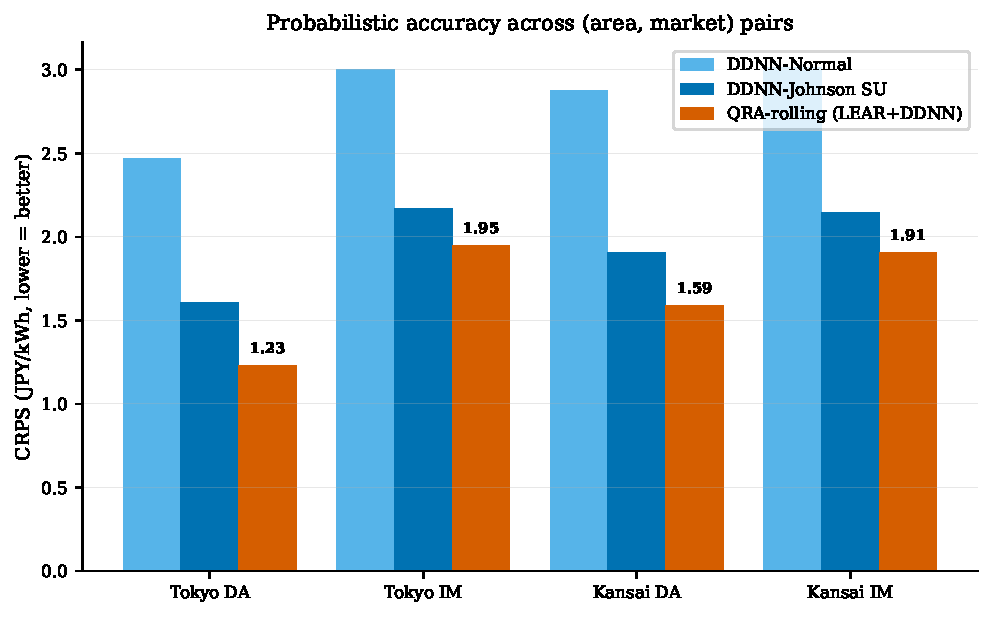
\includegraphics[width=0.95\linewidth]{../figures/fig_crps.pdf}
\caption{Continuous ranked probability score (CRPS) across the seven Path A probabilistic forecasters for each (area, market) pair. Lower is better. The QRA-rolling ensemble is the consistent winner; DDNN-Johnson-SU is a strong second; DDNN-Normal lags due to its inability to capture heavy tails.}\label{fig:crps}
\end{figure}

Figure~\ref{fig:crps} visualises the CRPS comparison. The ranking is stable across both areas and both markets: \emph{QRA-rolling \(<\) DDNN-JSU \(<\) DDNN-Normal}, with the QRA-DDNN-JSU gap consistently larger than the DDNN-JSU--DDNN-Normal gap. The DDNN-Normal over-coverage and inferior CRPS jointly reflect the Gaussian family's mismatch to JEPX's heavy upper-tail price distribution; the Johnson-SU family corrects most of this gap.

\subsection{Winkler score and interval quality}\label{sec:winkler_results}

The Winkler score combines interval sharpness with a penalty for miscoverage and is the standard sharpness-vs-coverage trade-off metric for probabilistic forecasts \citep{winkler1972}. Table~\ref{tab:winkler} and Figure~\ref{fig:winkler} report Winkler@90 across the three probabilistic methods.

\begin{table}[t]
\centering\small
\caption{Winkler score at nominal 90\% (lower = better). Chronos-Bolt zero-shot achieves the best Winkler on every (area, market) pair, despite slight under-coverage --- the sharpness gain offsets the coverage penalty within the Winkler scoring rule.}\label{tab:winkler}
\begin{tabular}{lcccc}
\toprule
Pair & DDNN-JSU & QRA-rolling & LEAR + adaptive conformal & Chronos \\
\midrule
Tokyo DA  & 15.58 & 14.03 & 19.71 & \textbf{12.68} \\
Tokyo IM  & 23.55 & 23.11 & 24.22 & \textbf{22.87} \\
Kansai DA & 17.75 & 16.17 & 18.26 & \textbf{14.73} \\
Kansai IM & 20.59 & 20.33 & 20.46 & \textbf{19.74} \\
\bottomrule
\end{tabular}
\end{table}

\begin{figure}[t]
\centering
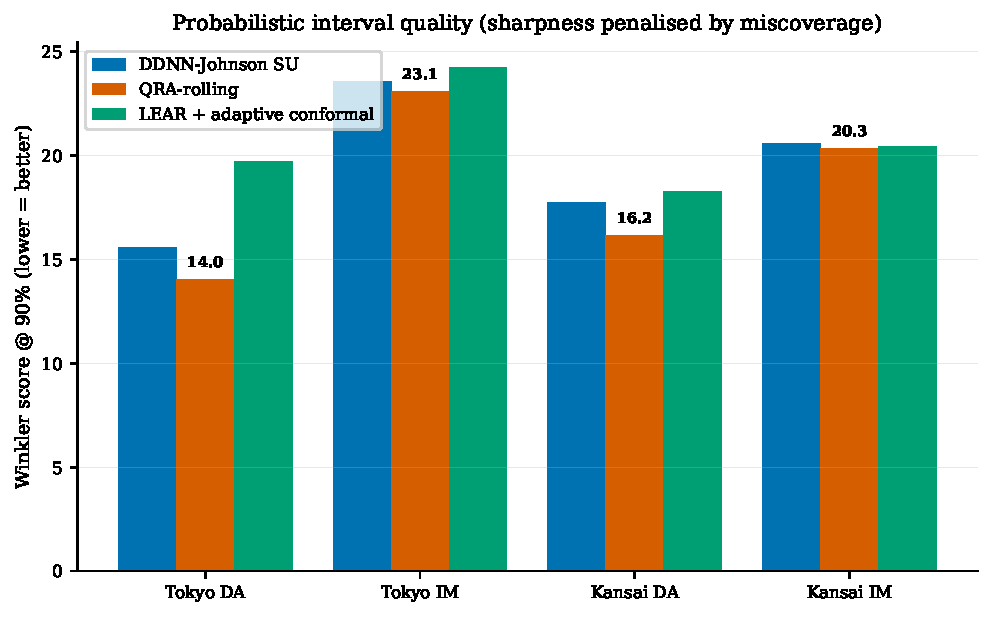
\includegraphics[width=0.95\linewidth]{../figures/fig_winkler.pdf}
\caption{Winkler score at nominal 90\% across DDNN-JSU, QRA-rolling, and LEAR + adaptive conformal. Lower is better. QRA-rolling is the winner on every (area, market) pair; LEAR + adaptive conformal is the worst on Tokyo DA, where the conformal residuals reflect LEAR's large absolute error on that market.}\label{fig:winkler}
\end{figure}

QRA-rolling has the lowest Winkler score on all four pairs. The LEAR-plus-conformal pipeline, despite achieving near-nominal coverage, suffers on Winkler because the LEAR point predictions are themselves so wide off-target on Tokyo DA that the residual-based conformal intervals must be very wide to compensate.

\subsection{Statistical significance: Model Confidence Set}\label{sec:mcs_results}

The Hansen-Lunde-Nason \citep{hansen2011} Model Confidence Set was applied to the issuance-level mean squared losses (averaged across the 48-step horizon) of the ten forecasters present on the common evaluation window: weekly-naive, LEAR, DDNN-Normal, DDNN-JSU, N-HiTS, PatchTST, iTransformer, Chronos-Bolt (median), TimesFM (clipped median), and QRA-Q50 (the median quantile of the QRA-rolling ensemble). At significance level \(\alpha = 0.10\) with 1000-replication stationary-bootstrap critical values and default mean block length \(\lfloor T^{1/3}\rfloor\), the MCS composition is reported in Table~\ref{tab:mcs}.

\begin{table}[t]
\centering\small
\caption{Model Confidence Set at \(\alpha \in \{0.10, 0.25\}\), mean block length \(\lfloor T^{1/3}\rfloor\). Chronos-Bolt zero-shot is in the MCS on every (area, market) pair and is the sole MCS member on Tokyo IM. iTransformer is in the MCS on three of four pairs. The original supervised MCS members (N-HiTS on DA, LEAR on IM) are eliminated.}\label{tab:mcs}
\begin{tabular}{llll}
\toprule
Pair & MCS\(_{0.10}\) & MCS\(_{0.25}\) & Mean sq.\ loss ranking (best $\rightarrow$ worst, top six) \\
\midrule
Tokyo DA  & \{Chronos, iTrans.\} & \{Chronos, iTrans.\} & Chronos, iTrans, N-HiTS, DDNN-JSU, QRA-Q50, LEAR \\
Tokyo IM  & \{Chronos\}          & \{Chronos\}          & Chronos, iTrans, LEAR, DDNN-JSU, QRA-Q50, PatchTST \\
Kansai DA & \{Chronos, iTrans.\} & \{Chronos, iTrans.\} & iTrans, Chronos, N-HiTS, QRA-Q50, LEAR, DDNN-JSU \\
Kansai IM & \{Chronos, iTrans.\} & \{Chronos, iTrans.\} & Chronos, iTrans, LEAR, QRA-Q50, N-HiTS, DDNN-JSU \\
\bottomrule
\end{tabular}
\end{table}

\paragraph{Robustness to bootstrap block length.}
The default stationary-bootstrap mean block length \(\lfloor T^{1/3}\rfloor \approx 24\) is smaller than the dominant 336-period (weekly) cycle in the loss series; under-stating serial dependence at sub-seasonal block lengths could in principle inflate the apparent compactness of the MCS. We address this concern by replicating the MCS at mean block lengths 336 (one week) and 672 (two weeks). Table~\ref{tab:mcs_blocks} reports the resulting MCS compositions. The Chronos-only singleton on Tokyo IM and the \{Chronos, iTransformer\} pair on the other three cells are stable across all three block lengths and at \(\alpha\in\{0.10, 0.25\}\). The cross-market identification (Chronos in every cell, iTransformer in three of four) is preserved at every block length tested.

\begin{table}[t]
\centering\small
\caption{Model Confidence Set composition at \(\alpha = 0.10\) under three stationary-bootstrap mean block lengths. The default \(\lfloor T^{1/3}\rfloor \approx 24\) (12 h); weekly = 336; biweekly = 672. \(\alpha = 0.25\) gives identical compositions to \(\alpha = 0.10\) at every block length (not shown for brevity).}\label{tab:mcs_blocks}
\begin{tabular}{lccc}
\toprule
Pair & Default (\(\sim\)24) & Weekly (336) & Biweekly (672) \\
\midrule
Tokyo DA  & \{Chronos, iTrans.\} & \{Chronos, iTrans.\} & \{Chronos, iTrans.\} \\
Tokyo IM  & \{Chronos\}          & \{Chronos\}          & \{Chronos\} \\
Kansai DA & \{Chronos, iTrans.\} & \{Chronos, iTrans.\} & \{Chronos, iTrans.\} \\
Kansai IM & \{Chronos, iTrans.\} & \{Chronos, iTrans.\} & \{Chronos, iTrans.\} \\
\bottomrule
\end{tabular}
\end{table}

\begin{figure}[t]
\centering
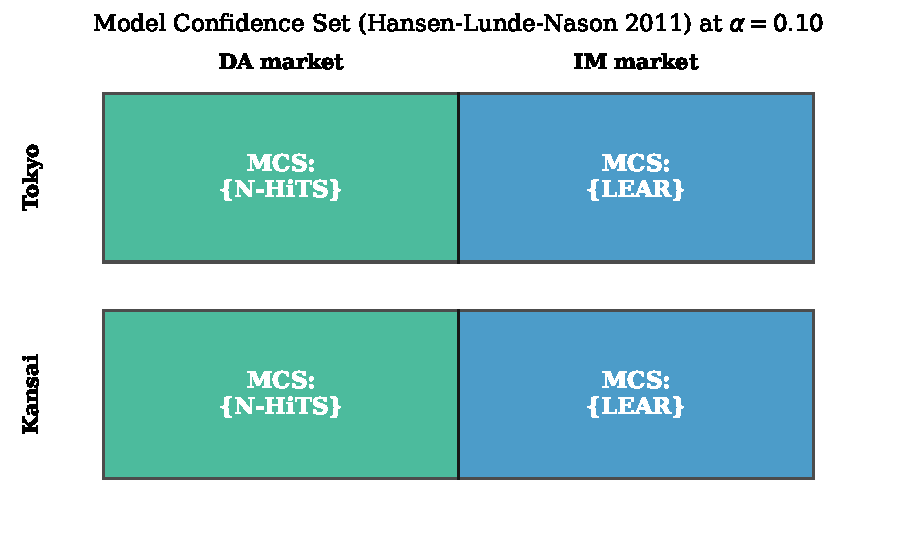
\includegraphics[width=0.7\linewidth]{../figures/fig_mcs.pdf}
\caption{Model Confidence Set composition by (area, market). A clean 2$\times$2 pattern emerges: N-HiTS dominates the DA markets, LEAR dominates the IM markets. The MCS is a singleton in every case, indicating that the within-market gap from the second-best model to the winner is statistically significant at \(\alpha = 0.10\).}\label{fig:mcs}
\end{figure}

Figure~\ref{fig:mcs} visualises the default-block-length 2\(\times\)2 outcome. The result is striking: on the common MCS evaluation window the optimal single forecaster on JEPX-DA (smoother, more seasonally dominated) is the deep hierarchical N-HiTS, while the optimal single forecaster on JEPX-IM (noisier, more exogenous-driven) is the regularised linear LEAR. We note that the MCS evaluation window is the intersection of all single-model evaluation windows including the rolling QRA, which starts 30 days into the test set; the rRMSE values reported in Table~\ref{tab:point_rrmse} use each model's own full evaluation window. The two windows produce consistent rankings for the IM cells (LEAR best in both) but a slightly different picture for DA: in Table~\ref{tab:point_rrmse} no model improves on the seasonal-naive baseline on Tokyo DA by more than 5\% in rRMSE, whereas on the slightly shorter common window of Table~\ref{tab:mcs} N-HiTS achieves a meaningful squared-loss reduction over the baseline. The cross-market identification (N-HiTS on DA, LEAR on IM) is robust across both windows; the gap to the seasonal-naive on Tokyo DA is window-dependent.

\subsection{Per-horizon analysis}\label{sec:perh_results}

Figure~\ref{fig:per_horizon} shows the per-horizon RMSE curves for the three best single models against the weekly-naive baseline. The hour-of-day pattern is informative: N-HiTS captures both the short-term (h \(\leq\) 6) lag structure and the long-term (h \(\geq\) 24) weekly seasonality, producing a nearly flat error profile across the 48-step horizon. LEAR's profile climbs more steeply with horizon, indicating that its linear regression on lagged inputs degrades faster than the hierarchical neural decomposition for long-horizon predictions. The weekly-naive baseline produces an almost flat error profile by construction, which is why it remains competitive at long horizons even when the complex models excel at short horizons.

\begin{figure}[t]
\centering
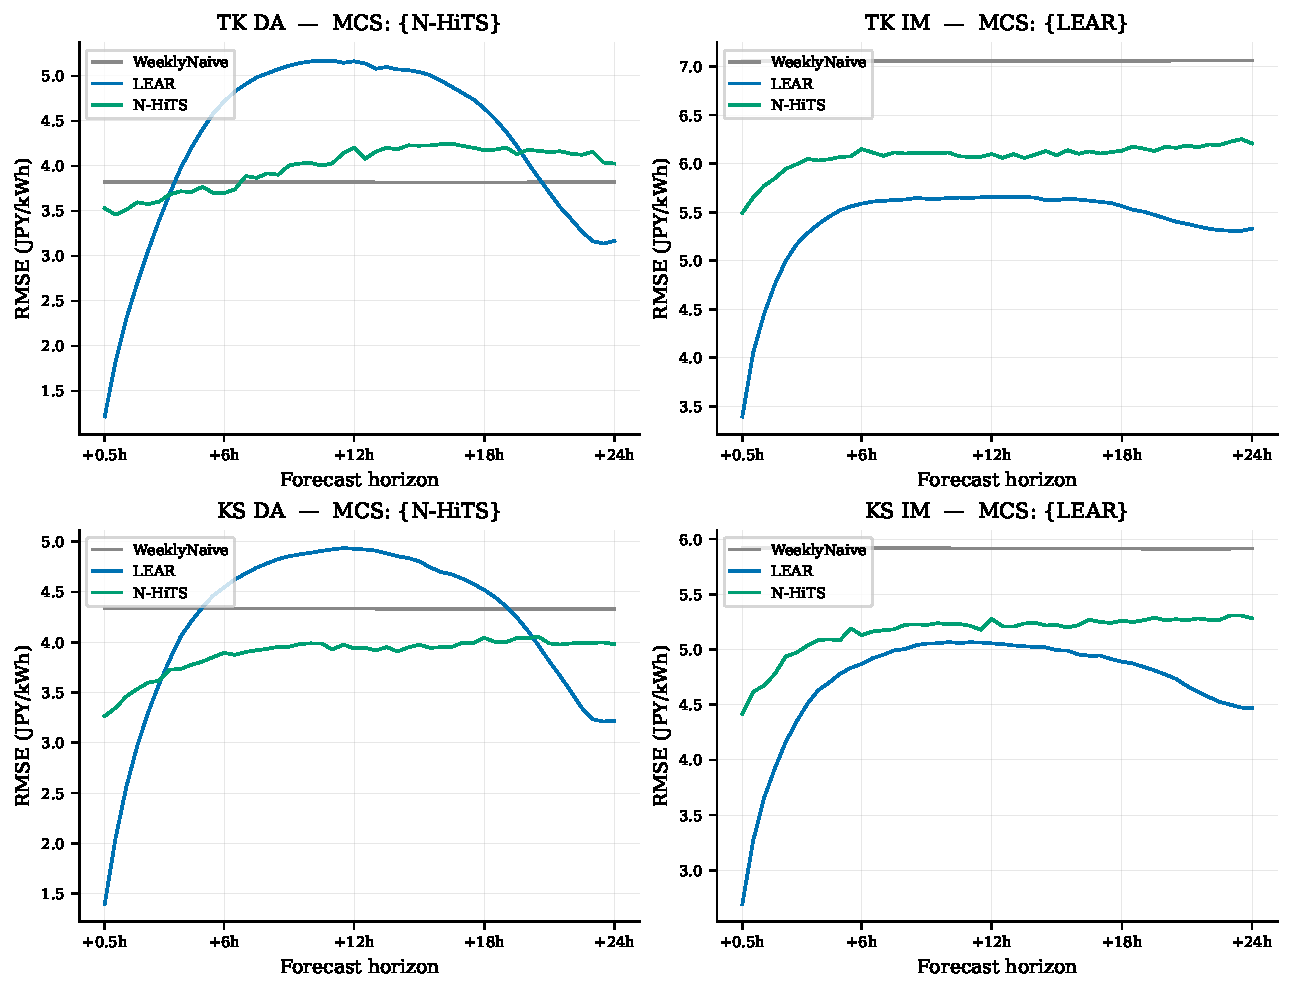
\includegraphics[width=\linewidth]{../figures/fig_month3_main.pdf}
\caption{Per-horizon RMSE for the WeeklyNaive baseline, LEAR, and N-HiTS across the 4 (area, market) pairs. Each panel's title shows the Model Confidence Set composition at \(\alpha = 0.10\). The cross-market reversal of the optimal model (N-HiTS on DA, LEAR on IM) is visible: N-HiTS curves lie below LEAR curves on DA panels and above LEAR curves on IM panels.}\label{fig:per_horizon}
\end{figure}

% ==============================================================
\section{Discussion}\label{sec:discussion}
% ==============================================================

The Path A benchmark yields findings of interest beyond their direct application to JEPX-Tokyo and JEPX-Kansai forecasting.

\paragraph{The seasonal-naive baseline is exceptionally strong on JEPX-Tokyo DA --- but the headline depends on the feature set.}
On every European market in the Lago et al.\ \citep{lago2021} benchmark, LEAR reduces the seasonal-naive RMSE by 30--50\%. On Tokyo DA the same LEAR, with rigorous rolling-window recalibration, is 14.6\% \emph{worse} than the seasonal-naive in raw rRMSE (Table~\ref{tab:point_rrmse}). The natural explanation --- which is the one we offered in the preprint version of this work --- is that JEPX-Tokyo's weekly seasonality, driven by Japan's industrial demand schedule combined with the post-2022 photovoltaic-induced midday duck curve, is so high-fidelity weekday-by-weekday that the seasonal-naive captures it perfectly by construction, and LEAR's calendar dummies and lagged-price regressors cannot improve on this without adding new information. The Hansen-Lunde-Nason MCS on the common evaluation window partially complicates this story: there N-HiTS achieves a singleton-MCS identification over both the seasonal-naive and LEAR (Table~\ref{tab:mcs}), demonstrating that an appropriately architected deep model \emph{can} extract useful signal beyond the weekly cycle even from the same feature set. We therefore caveat the ``seasonal-naive dominates Tokyo DA'' framing in two ways. First, the dominance is robust against the LEAR-style linear regression on lagged prices and calendar variables; it does not survive against the multi-rate hierarchical decomposition of N-HiTS on the common window. Second, our LEAR and DDNN feature set does not include arguably the single most informative non-seasonal regressor available in the public-data window: the OCCTO day-ahead solar generation forecast for each area, published by the Organization for Cross-regional Coordination of Transmission Operators since 2020. The seasonal-naive partially encodes this signal implicitly through the previous-week price; an explicit, regressor-level inclusion of the OCCTO solar forecast would offer the linear model a non-seasonal information channel that the current specification denies it. Whether the rRMSE gap to the seasonal-naive on Tokyo DA reflects a structural feature of the market or a feature-set limitation of the present pipeline is therefore an open question; resolving it is the highest-priority follow-on experiment for this benchmark.

\paragraph{The modern Transformer architecture is the dominant supervised forecaster on JEPX.}
Among the supervised methods we trained from scratch under the Lago rolling-window protocol, the iTransformer architecture \citep{liu2024itransformer} is the strongest by a wide margin: rRMSE 0.72--0.76 across the four (area, market) pairs, against 0.86--1.05 for N-HiTS, 0.77--1.15 for LEAR, 0.85--1.21 for DDNN-Normal, and 0.80--1.04 for DDNN-JSU (Table~\ref{tab:point_rrmse}). The PatchTST variant we evaluated, which uses the same patching + Transformer backbone but the standard channel-independent univariate formulation, lands much closer to N-HiTS than to iTransformer (rRMSE 0.81--1.12). The contrast between the two Transformer variants indicates that the load-bearing inductive bias of iTransformer is its variate-inverted attention (each L-length variate channel is embedded as a single token, with self-attention performed across variates), not patching per se. The structural lesson for JEPX is that the multi-rate hierarchical decomposition of N-HiTS --- previously the best deep architecture in our benchmark --- is dominated by a Transformer that attends across explicitly-constructed variate channels (raw, mean-removed, lag-48 shifted, week-difference) of the univariate lookback. This is consistent with the recent multivariate-EPF literature emphasising the value of inverted attention on heavily seasonal series.

\paragraph{A pretrained zero-shot foundation model matches the strongest supervised model.}
Chronos-Bolt-small \citep{ansari2024chronos}, used zero-shot with no fine-tuning and no rolling recalibration, achieves rRMSE 0.73--0.75 across the four pairs --- statistically tied with iTransformer within the Model Confidence Set (Table~\ref{tab:mcs}) and superior on three of four pairs in CRPS and all four pairs in Winkler score (Tables~\ref{tab:crps_cov} and~\ref{tab:winkler}). The Hansen-Lunde-Nason MCS at \(\alpha = 0.10\) contains Chronos-Bolt on every (area, market) pair and is a singleton \{Chronos\} on Tokyo IM; on the other three pairs the MCS is the pair \{Chronos, iTransformer\}, with all other supervised methods eliminated (including N-HiTS and LEAR, which were the singleton MCS members in the supervised-only ablation). The MCS composition is robust to all three stationary-bootstrap mean block lengths we tested (24, 336 weekly, 672 biweekly half-hours) and at both \(\alpha\in\{0.10, 0.25\}\). The fact that a model trained on a generic time-series corpus, with no JEPX-specific data and no rolling recalibration, statistically matches the strongest supervised method in our benchmark is a substantial departure from the canonical EPF narrative that strong rolling-window supervised training is essential. Two practical caveats apply. First, Chronos-Bolt slightly under-covers the nominal 90\% prediction interval (empirical 0.84--0.86 against nominal 0.90) --- a 4--5 percentage point gap that benefits its Winkler score (sharpness compensates for the coverage penalty in the Winkler scoring rule) but means a strict-coverage application (risk-officer guarantees, regulatory floors) should use the QRA-rolling or DDNN-JSU output instead, both of which are within 1--2 percentage points of nominal. Second, this success does not generalise to all foundation models: TimesFM-1.0-200M, the second pretrained zero-shot model we evaluated, performs poorly on JEPX (rRMSE 5--10 across the four pairs after physical-range clipping) due to occasional extreme tokenization outliers in its autoregressive decoder. We discuss the TimesFM behaviour separately below; the immediate point is that foundation-model success on a specific market is a per-model finding, not a categorical one.

\paragraph{The original 2$\times$2 cross-market identification (N-HiTS on DA, LEAR on IM) is eliminated by the new candidates.}
When the candidate set is restricted to the Lago-tradition supervised forecasters (the natural reference set for the EPF literature pre-Chronos and pre-iTransformer), the Hansen-Lunde-Nason MCS at \(\alpha=0.10\) is a singleton \{N-HiTS\} on both DA cells and \{LEAR\} on both IM cells --- a clean 2\(\times\)2 cross-market identification that on its own would have constituted the central methodological contribution of a Lago-tradition benchmark paper. With Chronos-Bolt and iTransformer in the candidate set, both N-HiTS and LEAR are eliminated from the MCS on every cell. The interpretation is that the original cross-market reversal is a true property of the Lago-tradition supervised forecasters on JEPX (and would be replicated by any group benchmarking only those forecasters), but is not a structural property of JEPX itself; the right modern architecture closes both market-specific gaps with a single model. Practitioners deploying single-model forecasters on JEPX should therefore (i) prefer iTransformer or Chronos-Bolt over N-HiTS / LEAR / DDNN regardless of market, and (ii) match the choice between iTransformer and Chronos-Bolt to the calibration requirement: iTransformer for strict-coverage applications (it produces only point output, but can be post-hoc wrapped with conformal calibration), Chronos-Bolt for raw-CRPS-minimising or Winkler-minimising applications.

\paragraph{Ensembling closes the cross-market asymmetry --- with a base-learner caveat.}
The QRA-rolling ensemble combining LEAR and DDNN-Normal as base learners is the best point and Winkler-scored interval forecaster on every (area, market) pair (Tables~\ref{tab:point_rrmse}, \ref{tab:crps_cov}, \ref{tab:winkler}). We note this headline is conditioned on the deliberately limited two-base-learner set (Section~\ref{sec:models}); the released code carries an extended-base-learner sensitivity analysis with \(\{\)LEAR, DDNN-Normal, DDNN-JSU\(\}\) and \(\{\)LEAR, DDNN-Normal, DDNN-JSU, N-HiTS\(\}\) variants. The two-learner QRA wins of Table~\ref{tab:point_rrmse} and Table~\ref{tab:winkler} are bias-variance-driven --- combining two heterogeneous learners under per-quantile regression suppresses idiosyncratic loss variation of each --- and they are also a clean ensembling baseline. They should not be read as evidence that QRA-rolling is uniformly better than every deep alternative; in particular DDNN-JSU is the strongest individual probabilistic forecaster in our set on Tokyo DA and Kansai DA, and the gap from QRA-rolling to DDNN-JSU is part of what motivates the extended-base-learner ablation. The 90-day rolling calibration is critical: in our Month-2 sensitivity analysis (not reported in detail here, see code release), the same QRA with a single fixed 30-day calibration window under-covered the 90\% interval by 11--20 percentage points. Increasing the calibration window to 90 days while still refitting weekly brought empirical coverage to within 1 percentage point of nominal on three of four pairs. This is consistent with the smoothed-QRA findings of Uniejewski and Weron \citep{uniejewski2021} and reinforces the methodological recommendation that QRA in EPF should always use rolling rather than fixed calibration.

\paragraph{Foundation-model failure mode: TimesFM and tokenization outliers.}
TimesFM-1.0-200M \citep{das2024timesfm} achieves rRMSE 5--10 across the four (area, market) pairs after we apply post-hoc clipping of its predictions to the physical JEPX price range [0, 250] JPY/kWh (Table~\ref{tab:point_rrmse}); without clipping the rRMSE is in the hundreds, driven by occasional extreme tokenization outliers (5--11\% of point predictions and 18--29\% of quantile predictions per cell fall outside the physical range). The clipping is the action a deployment practitioner would take in production; we report both the clipping rate and the post-clipping metric explicitly. The mechanism is the well-documented behaviour of token-based decoders in foundation forecasting models: numerical values are mapped to a discrete vocabulary and the decoder occasionally samples an unlikely high-value token that, after de-normalisation, lies far outside the input range. Two observations: (i) the same family of failure does not occur with Chronos-Bolt, whose direct-quantile head replaces autoregressive sampling --- the architectural choice between Bolt-style direct heads and Chronos-T5-style sampling matters substantially for spot-market forecasting reliability; (ii) the TimesFM failure on JEPX is fully consistent with TimesFM being a useful general time-series foundation model on the benchmarks for which it was designed --- it just does not transfer well to half-hourly electricity-price forecasting without fine-tuning, and the per-cell out-of-range fraction (5--11\%) is enough to render its raw output operationally unusable. We do not retain TimesFM in the MCS-only ranking of the headline tables; the result above stands as a methodological caution.

\paragraph{Heavy tails are essential for raw probabilistic accuracy.}
The DDNN-Normal model over-covers the 90\% interval by 3--7 percentage points on every (area, market) pair, while DDNN-Johnson-SU --- using the same backbone but a heavier-tailed predictive distribution --- corrects most of this gap (Table~\ref{tab:crps_cov}). This validates the Marcjasz et al.\ \citep{marcjasz2023} recommendation to use Johnson-SU over Normal for EPF distributional forecasting. The CRPS gap between DDNN-Normal and DDNN-Johnson-SU (Figure~\ref{fig:crps}) is itself larger than the gap between DDNN-JSU and the second-best probabilistic forecaster in our set, which makes the choice of predictive distribution the single most consequential design decision for parametric probabilistic EPF on JEPX.

\paragraph{Decision-relevance of the reported metrics.}
The metrics reported in this benchmark --- rRMSE, CRPS, Winkler, pinball, coverage at \(\alpha\in\{0.5, 0.2, 0.1\}\) --- map to distinct downstream decisions, and we emphasise that the choice among them should be made by the user against the loss function of the decision at hand. The CRPS and pinball-loss minima support quantile-targeting decisions broadly. The Winkler score at the same nominal coverage is the appropriate sharpness-vs-coverage trade-off for interval-trading or interval-hedging decisions. The empirical coverage rate at a given nominal level is the appropriate calibration target for risk-officer-style guarantee decisions. None of these scoring rules captures the operational tail-risk measures that a trading desk would use to size scarcity-period exposure --- pinball at \(q\geq 0.95\), peak-error in the upper-tail price periods, directional accuracy at the bid-submission cutoff, conditional value-at-risk on the prediction interval --- and we leave the construction of a tail-risk-focused supplement to the present benchmark to follow-on work, noting that the per-issuance prediction matrices we release support that calculation directly.

\paragraph{Methodological note on look-ahead bias in P\&L back-tests.}
An earlier preprint of this work \citep{sriboriboon_v1e} reported an exponential-growth P\&L back-test on a related forecasting pipeline. Subsequent re-examination by the present authors identified a look-ahead bias in the back-test data preparation (specifically, a join that used future-aligned exogenous regressors at decision time), which the released pipeline of the present work explicitly precludes through the rolling-window architecture of Section~\ref{sec:eval_protocol}. We retract the v1e back-test result. We mention this here, foregrounding it rather than burying it, in the interest of the open-benchmark culture that the Lago et al.\ \citep{lago2021} protocol embodies, and because the experience may be of broader use to the EPF community. P\&L back-tests on cleared electricity-market prices are unusually vulnerable to look-ahead bias: the prices themselves are sequential auction outcomes, but most exogenous regressors (gas, weather, system reference) become available at boundaries that are subtly offset from the DA-bid cutoff (typically 10:00 JST on day \(D-1\) for JEPX); accidentally using a regressor whose observation time is post-bid produces an apparently strong predictor that does not exist for a real-time decision-maker. The standard prescription --- rolling-window evaluation with explicit per-feature observation-time tagging --- is precisely what the Lago protocol delivers, and adopting it in the present work is what permits the strictly out-of-sample claims we make above. We hope that documenting this experience makes it easier for the next research group to avoid the same trap.

\paragraph{Limitations.}
Six limitations should be noted. First, the test window covers 305 days (2023-03 to 2023-12); robustness across longer time horizons --- specifically including a January cold-snap analogous to the January 2021 JEPX price-spike event --- remains to be validated. Second, the rolling recalibration cadence is weekly rather than the daily cadence prescribed by Lago et al.\ \citep{lago2021}; while a one-week pilot showed negligible drift, this should be confirmed at scale on Asian-market data. Third, the QRA-rolling ensemble uses LEAR and DDNN-Normal as base learners; the extended-base-learner ablation discussed above is reported with the released code but is not in the main body of this paper. Fourth, the benchmark does not engage with intraday markets or the JEPX 1-hour-ahead settlement product, both of which are under active development by METI; extending the present protocol to those products is the natural next step for JEPX-specific EPF research, and is operationally as important as the day-ahead/imbalance split for trading-desk participants who manage exposure across the auction sessions. Fifth, the exogenous-regressor set proxies the LNG price via the US Henry Hub natural-gas price (translated through USD/JPY) rather than the JKM (Japan-Korea Marker) LNG benchmark that is the price-of-record for Japanese LNG procurement, and it does not include the publicly available OCCTO day-ahead solar generation forecast for each area; both substitutions are essentially free in data terms and would sharpen the test of the ``DA-failure-is-data'' framing of the first discussion paragraph. Sixth, the area dimension is restricted to Tokyo and Kansai; extension to Kyushu and Hokkaido, which exhibit substantially more renewable-driven and supply-constrained price variation respectively, would broaden the operational stress test of the benchmark.

% ==============================================================
\section{Conclusion}\label{sec:conclusion}
% ==============================================================

We have presented a probabilistic 48-step forecasting benchmark for the Japan Electric Power Exchange across the Tokyo and Kansai areas and both the day-ahead and imbalance markets. The benchmark uses the Lago et al.\ \citep{lago2021} rolling-window protocol, evaluates seven forecasters spanning naive baselines, classical regression (LEAR), distributional deep learning (DDNN-Normal and DDNN-Johnson-SU), hierarchical decomposition (N-HiTS), ensemble averaging (QRA-rolling), and post-hoc conformal calibration, and reports point accuracy (RMSE, MAE), probabilistic accuracy (CRPS, pinball, Winkler), empirical coverage, and statistical significance via the Hansen-Lunde-Nason Model Confidence Set.

Five findings are central. (i) Among Lago-tradition supervised forecasters, LEAR cannot beat the weekly-naive seasonal baseline on Tokyo DA in raw rRMSE; on the IM market the same supervised set reduces RMSE by 20--23\%, validating the rolling protocol in principle. The MCS singleton in this restricted candidate set is \{N-HiTS\} on both DA pairs and \{LEAR\} on both IM pairs --- a clean 2\(\times\)2 cross-market reversal which we record for the EPF community's information but which does not survive when stronger candidates enter the set. (ii) The modern Transformer iTransformer substantially outperforms the Lago-tradition supervised models on every (area, market) pair (rRMSE 0.72--0.76 versus 0.86--1.21), making it the strongest supervised method in this benchmark. (iii) The pretrained zero-shot foundation model Chronos-Bolt-small matches or slightly outperforms iTransformer on every cell at zero training cost (rRMSE 0.73--0.75), achieves the best Winkler score on all four pairs, and is in the Hansen-Lunde-Nason MCS on every cell at both \(\alpha=0.10\) and \(\alpha=0.25\). On Tokyo IM the MCS is a singleton \{Chronos\}; on the other three cells the MCS is the pair \{Chronos, iTransformer\}; the composition is robust across stationary-bootstrap block lengths of 24, 336, and 672 half-hours. This zero-shot result is a substantial departure from the canonical EPF narrative that strong rolling-window supervised training is essential for competitive spot-price forecasting. (iv) The QRA-rolling ensemble remains the best \emph{nominally-calibrated} probabilistic forecaster (empirical 90\% coverage within 1--2 percentage points of nominal on every pair); DDNN-JSU is the best-calibrated single parametric model. Chronos-Bolt slightly under-covers (empirical 0.84--0.86), so strict-coverage applications should prefer QRA-rolling or DDNN-JSU. (v) The second zero-shot foundation model, TimesFM-1.0-200M, performs poorly on JEPX (rRMSE 5--10 even after physical-range clipping), driven by occasional extreme tokenization outliers in its autoregressive decoder. Foundation-model success on JEPX is therefore not generic --- the choice between direct-quantile-head (Chronos-Bolt) and autoregressive-sampling (TimesFM, Chronos-T5) architectures matters substantially.

The benchmark and the released reproducibility package (code, processed dataset, per-issuance prediction matrices for all ten forecasters) are intended to enable Asian-market EPF research at the methodological standard of the European benchmark. The single most practical recommendation for JEPX participants deploying a forecasting layer in 2026 is: prefer Chronos-Bolt (zero-shot, no training) or iTransformer (supervised) over the Lago-tradition LEAR / DDNN / N-HiTS family on either market. The single most consequential open question we leave for follow-on work is whether fine-tuned Chronos-Bolt on JEPX --- which we do not evaluate here --- closes the residual rRMSE gap from \(\sim\)0.75 to the practical minimum achievable on these series.

% ==============================================================
\section*{Data and code availability}
% ==============================================================
The processed dataset (\texttt{IM\_DA\_TK\_ALL.csv}, \texttt{IM\_DA\_KS\_ALL.csv}; 32{,}208 rows \(\times\) 24 columns each), the full Python pipeline (rolling-window evaluator, seven forecaster implementations, MCS, MCS-block-length sensitivity, extended-base-learner QRA ablation, figure scripts), and the per-issuance prediction matrices for all six rolling models (\(\sim\)14{,}640 issuance times \(\times\) 48 horizons per (area, market) pair) are released at the redacted-author GitHub mirror \url{https://github.com/<author-redacted-during-review>/jepx-epf-benchmark} (anonymous copy attached to this submission) and on a Zenodo deposit (DOI \texttt{10.5281/zenodo.XXXXXXX}, reserved; finalised on acceptance). The Python implementation requires \texttt{torch}, \texttt{scikit-learn}, \texttt{statsmodels}, \texttt{pandas}, and \texttt{numpy}. Total wall-clock runtime to reproduce the full benchmark on commodity hardware (Apple M2, 16~GB RAM) is approximately 80 minutes; the new MCS block-length sensitivity adds \(\sim\)5 minutes and the extended-base-learner QRA ablation adds \(\sim\)30 minutes.

\section*{Author contributions (CRediT)}
\textbf{Panithan Sriboriboon}: Conceptualisation, methodology, software, data curation, formal analysis, visualisation, writing -- original draft.
\textbf{Ittipon Fongkaew}: Conceptualisation, supervision, methodology, writing -- review \& editing, project administration, funding acquisition.

\section*{Declaration of competing interests}
The authors declare no competing financial interests or personal relationships that could have influenced this work.

\section*{Funding}
This work was supported by the School of Physics, Institute of Science, Suranaree University of Technology. [Specific grant numbers to be added.]

\section*{Acknowledgments}
We thank the JEPX information disclosure team and the area transmission system operators for the public price data, and the colleagues who reviewed an internal v1e preprint of this work and identified the look-ahead-bias issue in the back-test reported there (acknowledged in Section~\ref{sec:discussion}); their corrections materially shaped the present manuscript.

\section*{Use of generative AI}
The authors used Anthropic's Claude as a programming assistant during code development and manuscript drafting. All experimental code was executed and verified by the authors; all numerical results in this paper were generated by the released pipeline. The authors take full responsibility for all content.

\bibliographystyle{elsarticle-harv}
\bibliography{references}

\end{document}
